\chapter{Evaluation}
\label{c:evalu}

In this chapter, we present the end-to-end evaluation of our system.
At first, we discuss the evaluation datasets and ground truth annotation.
Next, we present the quantitative results for both computation time and accuracy.
Finally, we conclude this chapter with evaluation of our system using a public dataset.

\section{Evaluation datasets}
\label{s:eval}
To our best knowledge, there is not much research on sensor fusion in the context of traffic light detection, especially for pedestrian navigation. 
As a result, we did not find public datasets combining traffic lights video and inertial sensor data. 
Hence, we collected our own ground truth data using an Android app, that we discussed in \S\ref{s:app}.
\ref{f:ground_truth} shows the ground truth data collection using our Android app.

\begin{figure}[ht]
\centering
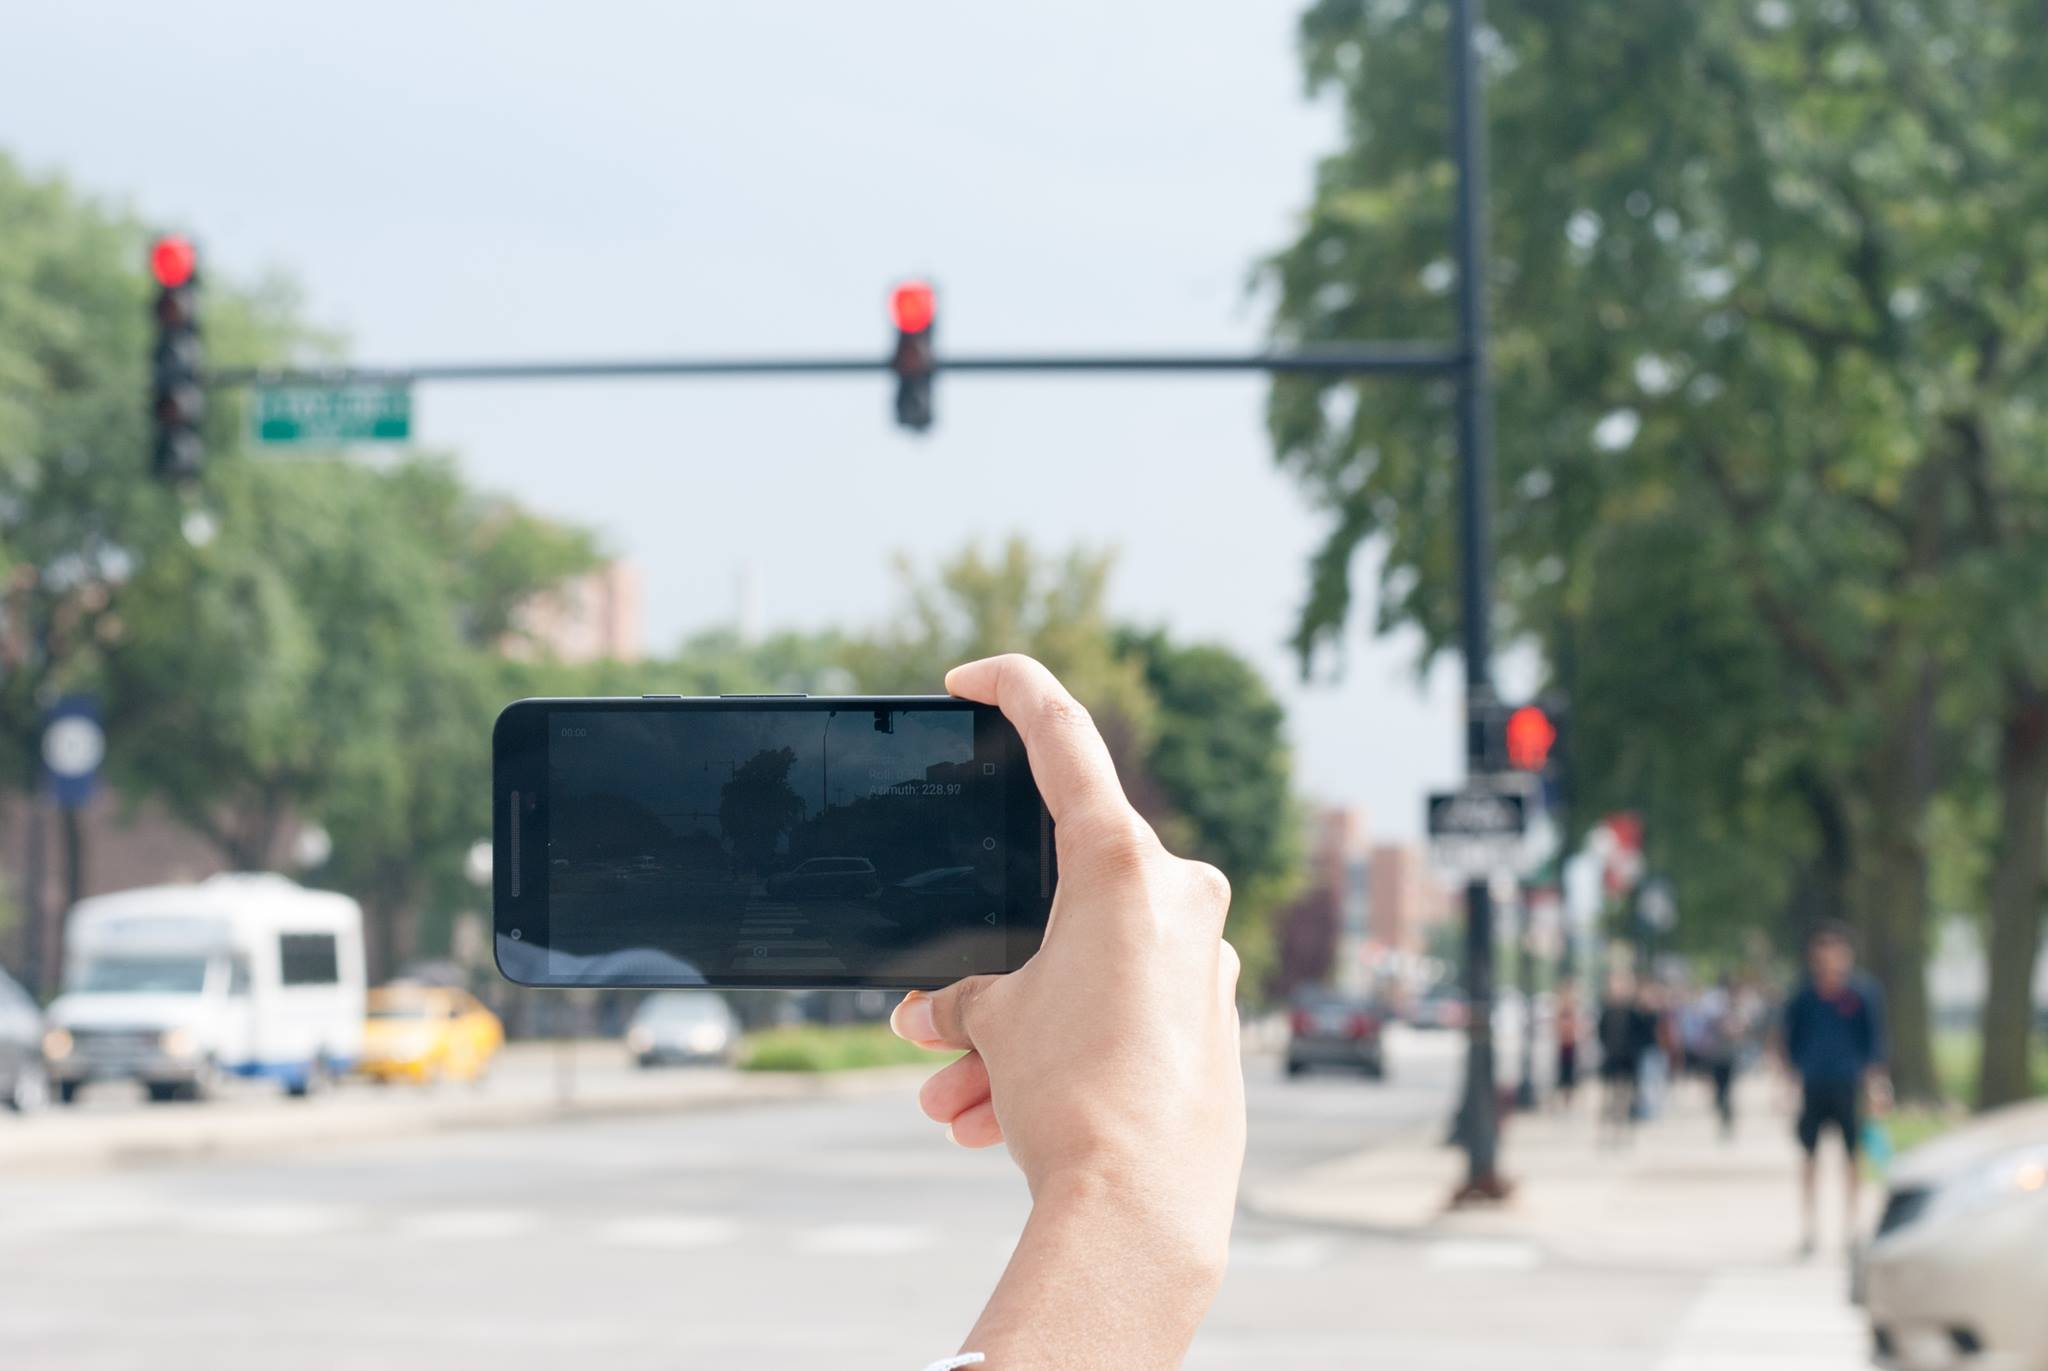
\includegraphics[width=5.2in]{images/ground_truth.jpg}
\caption{Ground truth data collection using Android app}
\label{f:ground_truth}
\end{figure}

% \todo{refer section or fig with the screenshot}.
We walked across several street crossings and recorded both video and sensor data simultaneously in various lighting conditions. 
For example, \ref{f:dataset} shows video frames for sunny, cloudy days and for night time. 
Here, we present our results for several 300 feet long walks.  
At the end of this chapter, we present an approximate evaluation of a public dataset that does not have sensor data. 
However, we emulate the effect of sensors by manual selection of a subpart of a video frame. 

\begin{figure}[ht!]
\centering
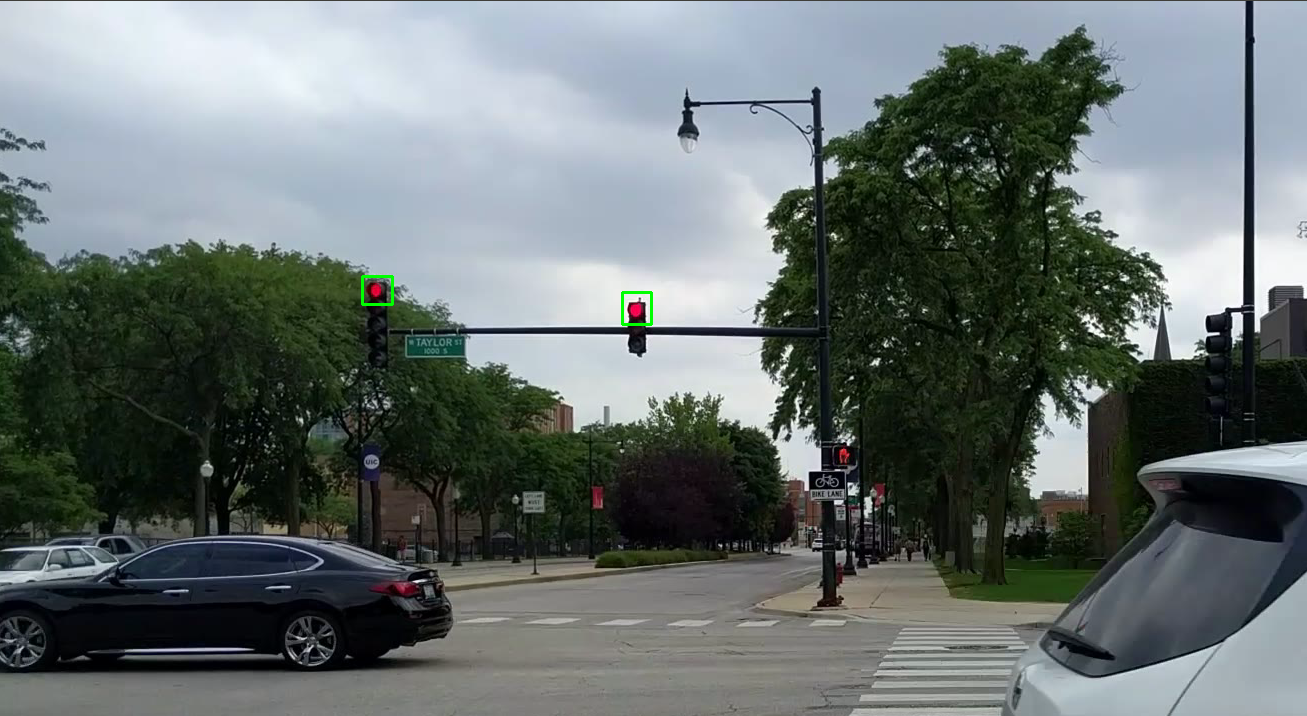
\includegraphics[width=5.2in]{images/annotation.png}
\caption{Interface for manual annotation. The green box provides the location of the traffic light in video frame.}
\label{f:annotate}
\end{figure}

\begin{figure}[!ht]
\centering
\subfloat[Sunny] {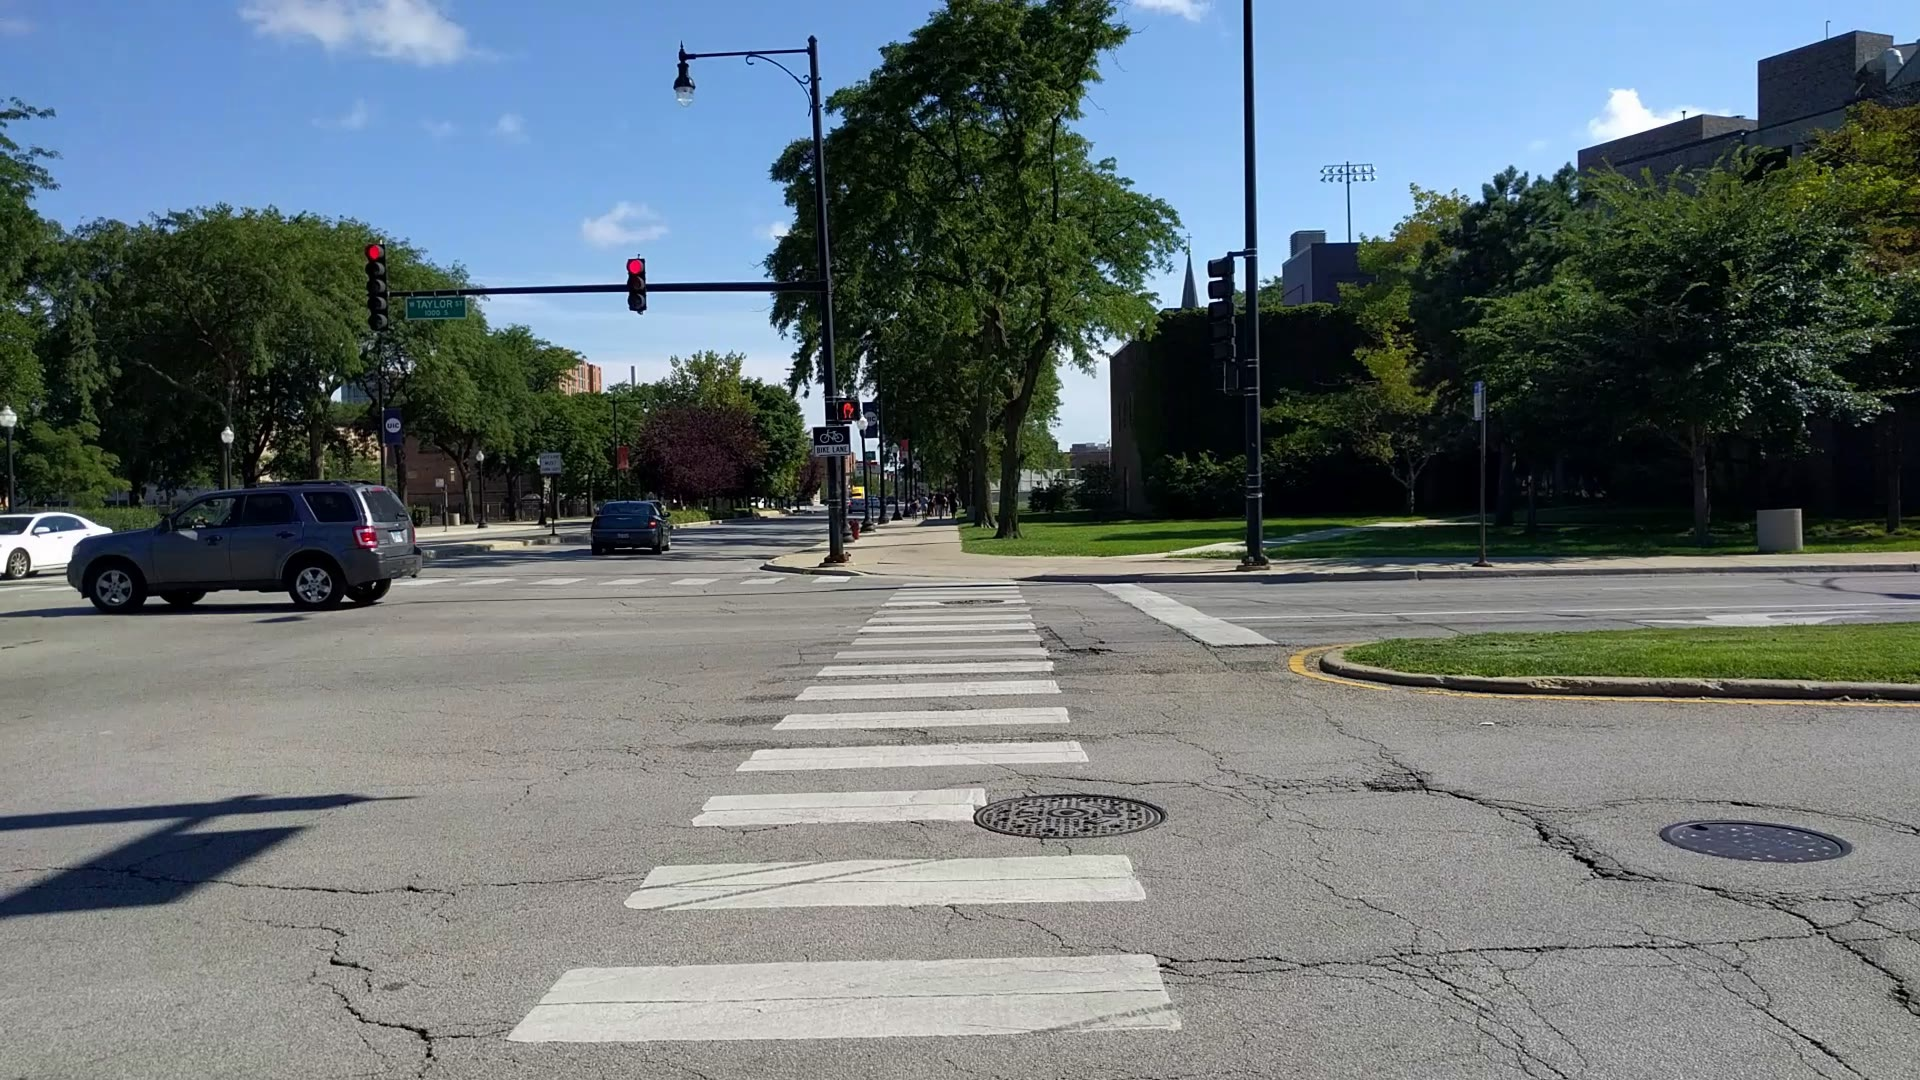
\includegraphics[width=3.2in]{images/sunny.jpg}}\\
\subfloat[Cloudy] {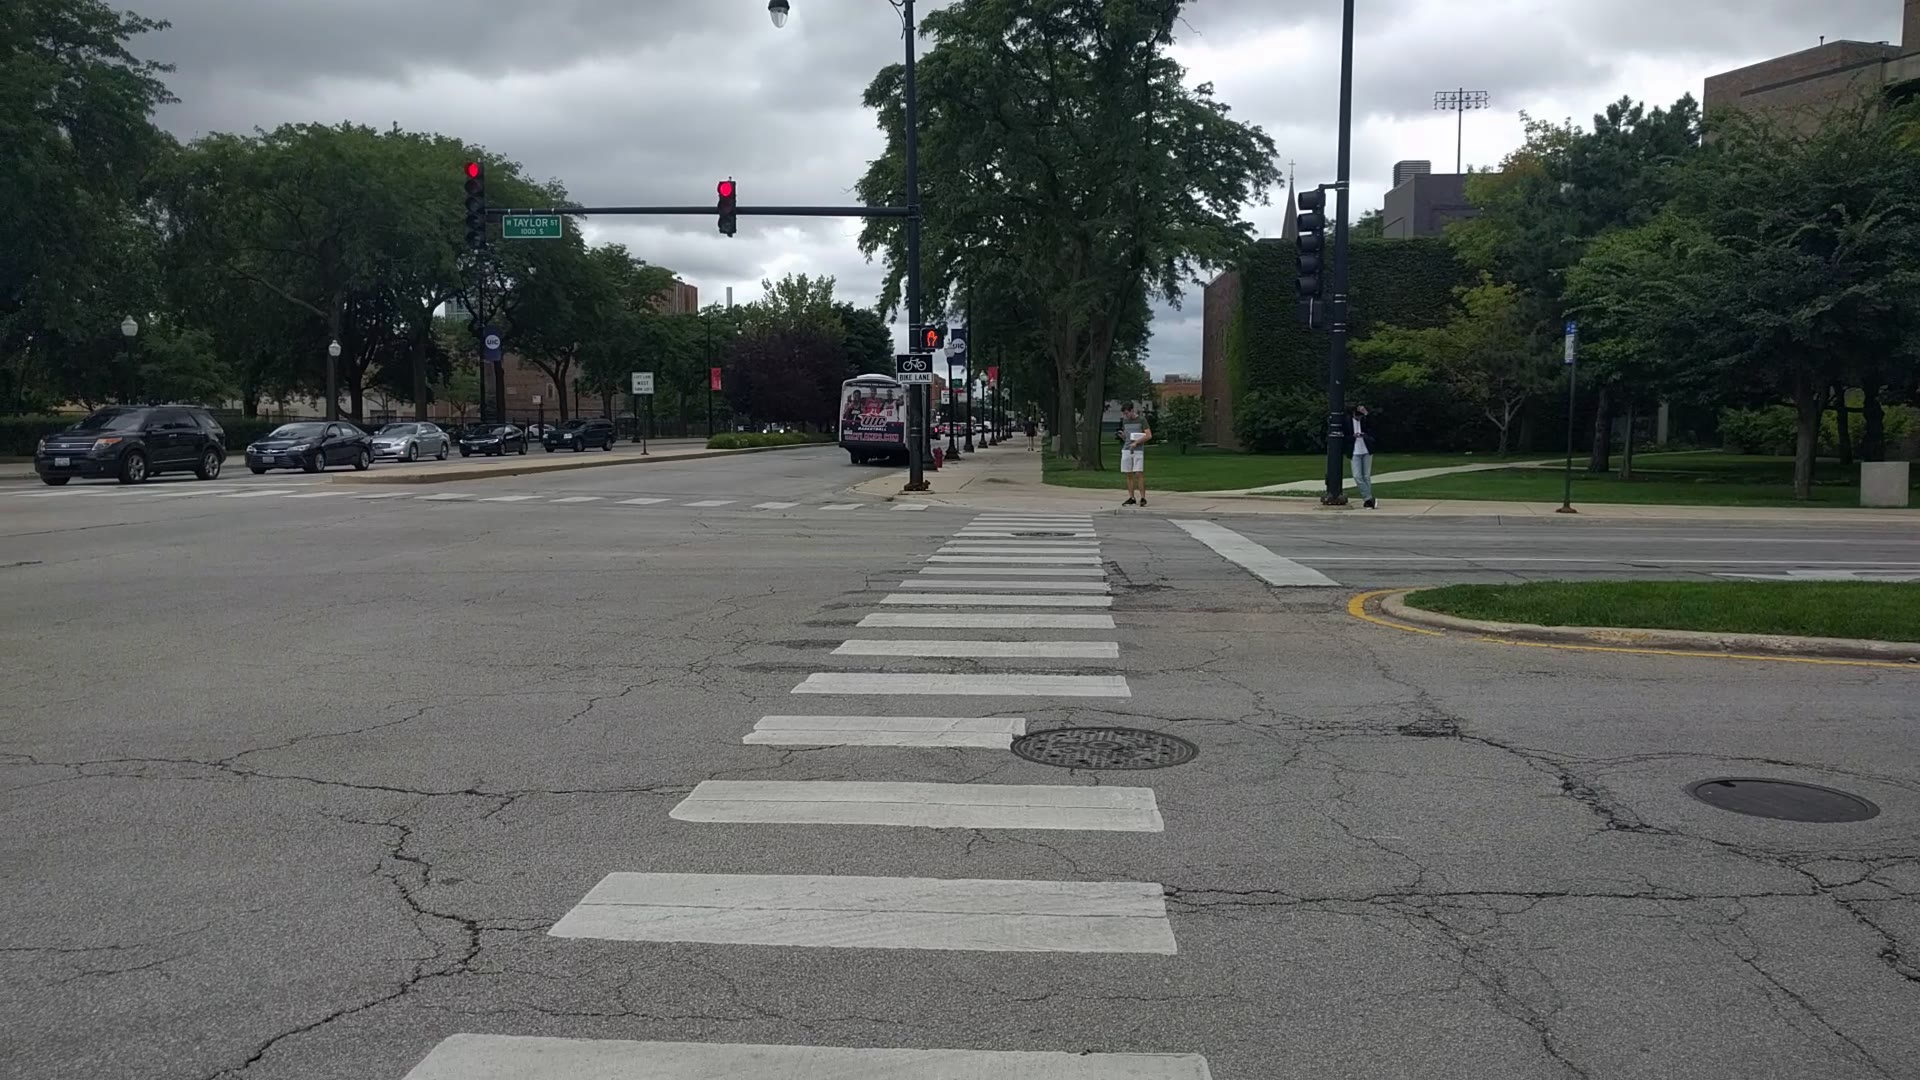
\includegraphics[width=3.2in]{images/cloudy.jpg}}\\
\subfloat[Night] {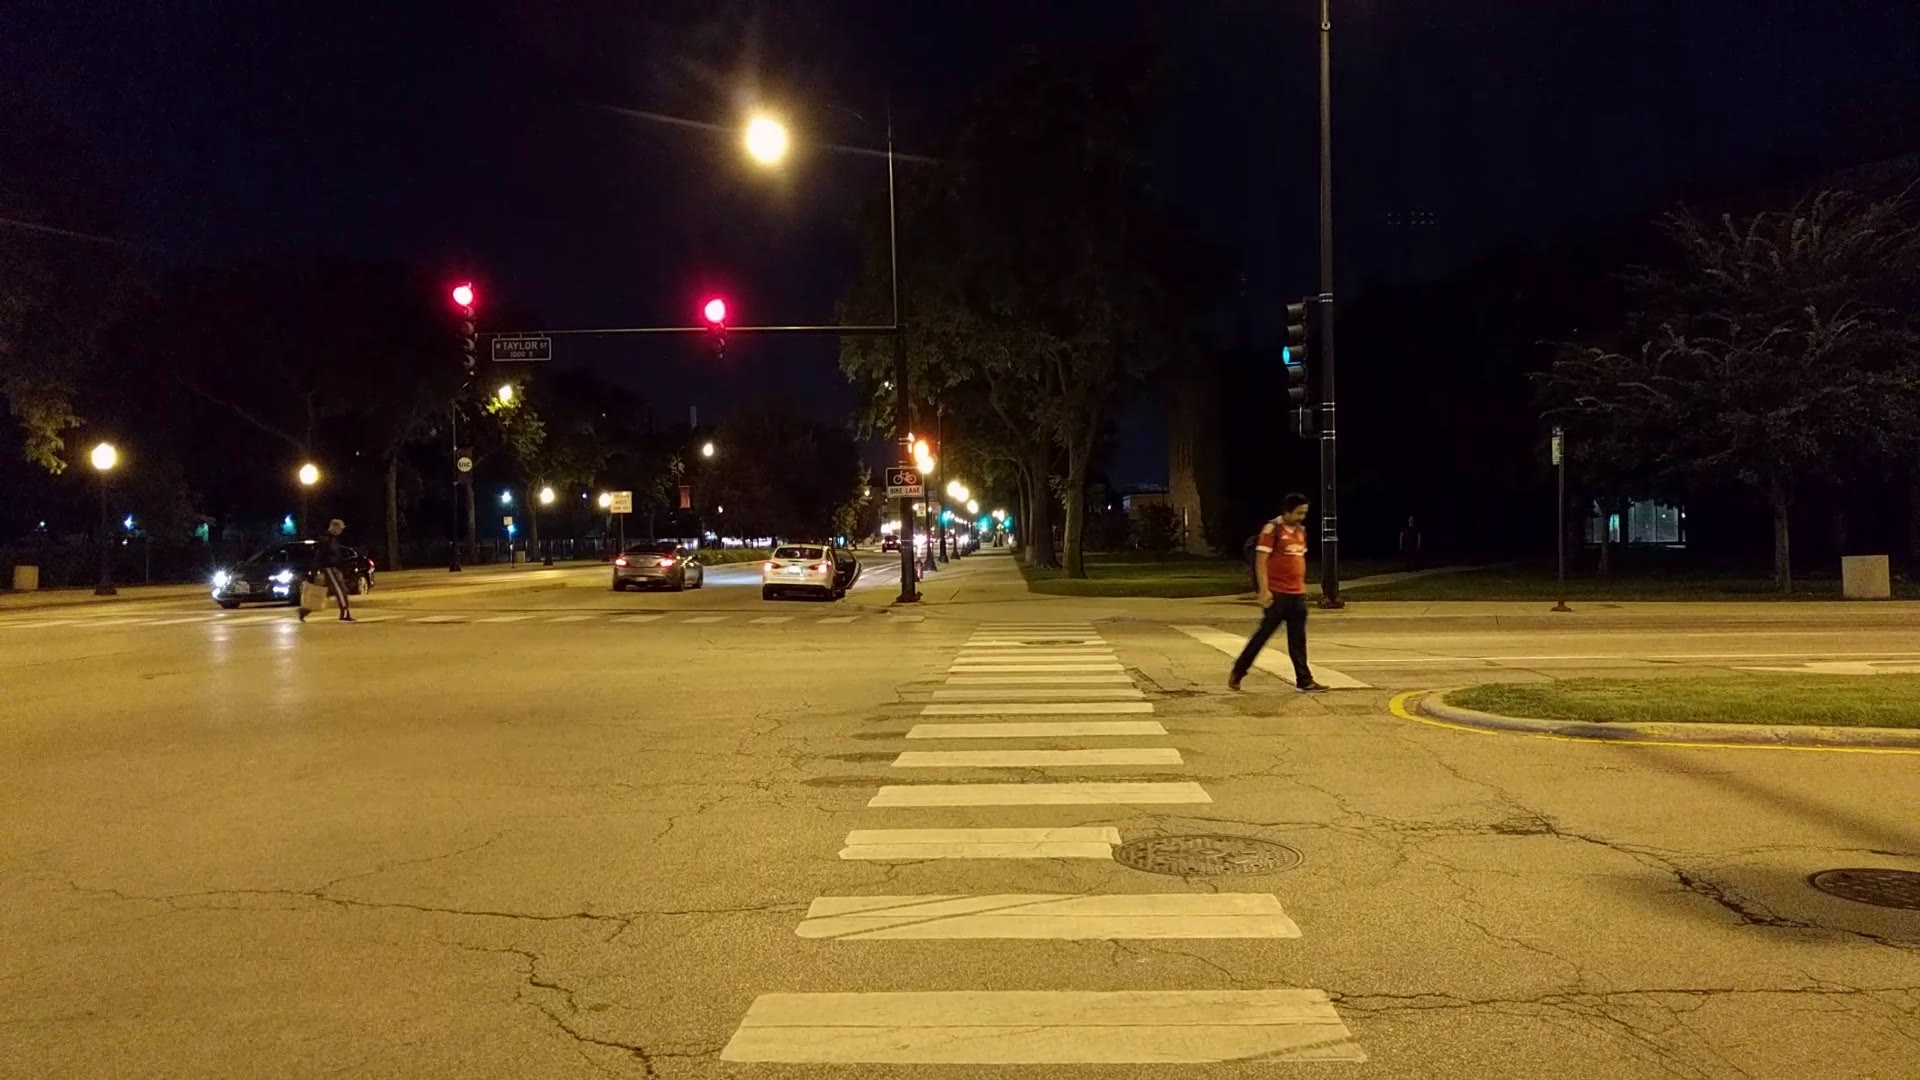
\includegraphics[width=3.2in]{images/night.jpg}}
\caption{Scene variation of recorded video.}
\label{f:dataset}
\end{figure}

\ref{t:dataset} shows the total no of frames and time duration of our dataset.

\begin{table}[ht!]
  \centering
  \caption{Description of the dataset.}
  \label{t:dataset}
  \rowcolors{2}{gray!25}{white}
  \begin{tabular}{  l  c  r r }
    \rowcolor{gray!50}
    Name & Frame Count & Time Duration \\
    \hline
    Walking w/ sensor (Sunny day) & 5905 & 3 mins 16 secs \\
    Walking w/ sensor (Cloudy day) & 6205 & 3 mins 26 secs \\ %& 807
    Walking w/ sensor (Regular day) & 6022 & 3 mins 20 secs \\%& 469
    Static w/ sensor (Regular day) & 1810 & 1 min \\%& 2014
    Walking w/ sensor (Night) & 6146 & 3 mins 24 secs \\
    \hline
  \end{tabular}
\end{table}

\section{Annotation}
We need the ground truth for traffic light positions on video frames in order to measure our system performance quantitatively.
Accordingly, we annotate the traffic light's positions manually by drawing a rectangle around the traffic lights at each video frame.
During annotation, we record the type of the traffic lights (i.e., red or green) and their positions with a bounding box.

\ref{f:annotate} shows the interface for manual annotation.
The green box provides the location of the traffic light and we annotate 0 for a red traffic light and 1 for a green traffic light.




\section{Computation time}
We collected data at different times of the day as we discussed in \S\ref{s:eval}.
In this section, we discuss the computation time of these datasets with and without the sensor fusion.

\subsection{Frame processing time}
\ref{f:cdf_cloudy} shows the computation time CDF for video frames for walking dataset with sensor movement in cloudy weather described in \ref{t:dataset}.
\begin{figure}[ht]
\centering
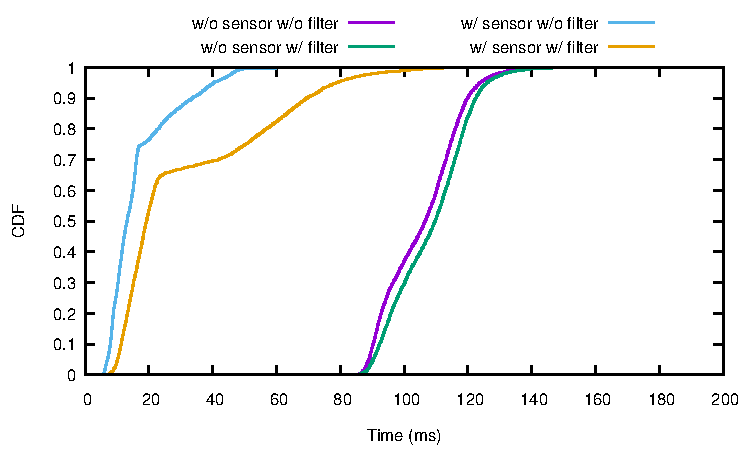
\includegraphics[width=5.2in]{plots/cloudy_cdf.pdf}
\caption{CDF of frame computation time for walking dataset with sensor movement in cloudy weather. The improvement of computation time is 5.29x if we use the sensor hints with the heuristic filter}
\label{f:cdf_cloudy}
\end{figure}
It shows that the median of the computation time without the sensor data and without the heuristic filters is 108.62ms.
On the other hand, the median computation time with the sensor and without heuristic filters is 13.11ms.
This is an improvement of 8.29x.
The median computation time with sensor and heuristic filters is 18.25ms.
There is a slight increase in frame processing time with the heuristic filters, but this is worthwhile as false detection rate reduces significantly with the heuristic filters.  
We discuss more about the accuracy and false detections in Section \S\ref{s:acc}

\ref{t:dataset_time} shows the median computation time for other datasets described in \ref{t:dataset}.
It shows that the average median computation time without sensor and without our heuristic filter is 113.11 ms.
On the contrary, the average median computation time with sensor and without our heuristic filter is 13.24 ms.
This is the average improvement is 8.54x.
The average median computation time with sensor and heuristic filter is 19.53 ms.
This gives the average improvement 5.79x, which is trivial decrease in computation time improvement, but this gives less false detection rate as we described earlier.

\begin{table}[!ht]
  \centering
  \caption{Median computation time (ms) with various settings for our dataset.}
  \label{t:dataset_time}
  \rowcolors{2}{gray!25}{white}
  \begin{tabular}{  l r r r r}
    \rowcolor{gray!50}
    Dataset Nane & W/o sensor & w/o sensor & w/ sensor  & w/ sensor \\
    \rowcolor{gray!50}
    & w/o filter & w/ filter & w/o filter & w/ filter\\
    \hline
    Walking w/ sensor (Cloudy) & 108.62 & 109.76 & 13.11 & 18.25 \\
    Walking w/ sensor (Sunny) & 112.74 & 113.67 & 13.32 & 19.82 \\
    Walking w/ sensor (Regular) & 110.43 & 114.12 & 13.89 & 20.17 \\
    Static w/ sensor (Regular) & 120.65 & 121.92 & 12.65 & 19.89\\
    \hline
    Avg. computation time (ms) & 113.11 & 114.87 & 13.24 & 19.53\\
    
  \end{tabular}
\end{table}

\subsection{Subimage processing time}
Processing a subpart of a video frame significantly reduces the computation time. 
We select a Region-Of-Interest (ROI) area within a frame with the sensor hints.
However, the ROI predicted from the sensor hints can be incorrect and we gradually increase the area of the rectangle.
We discussed the details about this in \S\ref{s:roi}.


\ref{f:recarea} shows the computation time with the increase of the ROI area in video frames.
It shows that the computation time increases as the area of the rectangle get larger.
For the same area, if the number of candidate pixels is high or the detected circle count is high then computation time increases.

\begin{figure}[ht!]
\centering
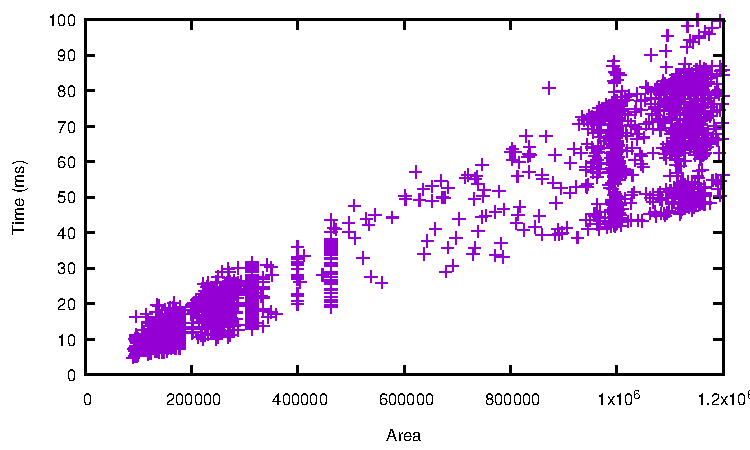
\includegraphics[width=5.2in]{plots/cloudy_recarea.pdf}
\caption{Computation time with the increase of the rectangle area. For the same rectangle area, computation time depends on the number of candidate pixels and detected circle count.}
\label{f:recarea}
\end{figure}



\subsection{Time for heuristic filtering}
We use a heuristic filter to reduce false positive in traffic light detection as we discuss at \S\ref{s:filter}.
The computational cost of the heuristic filter is very small.

\begin{figure}[ht!]
\centering
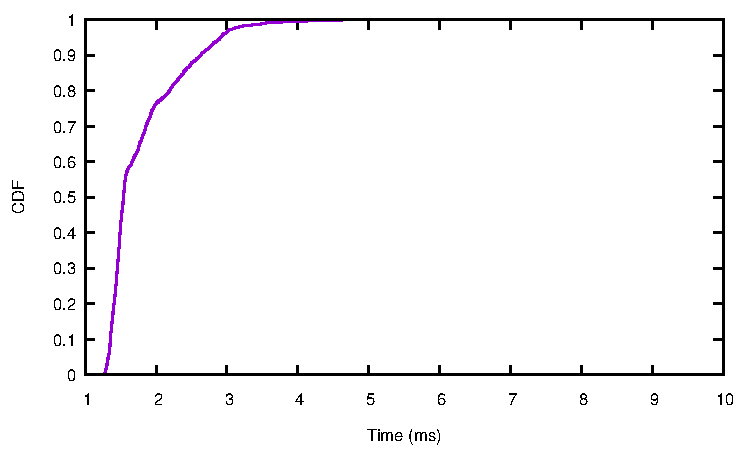
\includegraphics[width=5.2in]{plots/sunny_cdf_filter.pdf}
\caption{CDF of computation time for the heuristic filter.}
\label{f:cdf_fil}
\end{figure}

\ref{f:cdf_fil} shows the computation time of the heuristic filter.
The computation time depends on the number of circles detected on the frame.
If circle count is high, filtering need for all of these circles, so computation time gets higher.
\ref{f:cdf_fil} shows that the median computation time is 1.5 ms for the filtering. 





\section{Traffic lights detection accuracy}
\label{s:acc}
To demonstrate the robustness of the various traffic light scenarios, we recorded video at different lightening condition such as cloudy and sunny and at the different time of the day.
We walked along several crosswalks of few streets and the route had a total of 16 traffic lights.

\subsection{Confusion matrix}
\ref{t:con_nocrp} shows the confusion matrix for the traffic light decision when we do not consider the sensor hints of the smartphone.
\ref{t:con_crp} shows the confusion matrix considering the sensor hints in our dataset.

\begin{table}[ht!]
  \centering
  \caption{Confusion Matrix without sensor hints for our dataset. Each entry represents the decision number. Row and column entries are the associated accuracy.}
  \label{t:con_nocrp}
  \rowcolors{2}{gray!25}{white}
  \begin{tabular}{  l  c  c  r }
    \rowcolor{gray!50}
     & Detected Red & Detected Green &  \\
    \hline
    Actual Red & 1832 & 236 & 88.588\% \\
    Actual Green & 67 & 1155 & 94.5172\% \\
    \hline
    & 96.4718\% & 83.0338\% & 90.7902\% \\
    
  \end{tabular}
\end{table}

\begin{table}[ht!]
  \centering
  \caption{Confusion Matrix with sensor hints for our  dataset. Each entry represents the decision number. Row and column entries are the associated accuracy.}
  \label{t:con_crp}
  \rowcolors{2}{gray!25}{white}
  \begin{tabular}{  l  c  c  r }
    \rowcolor{gray!50}
     & Detected Red & Detected Green &  \\
    \hline
    Actual Red & 1952 & 116 & 94.3907\% \\
    Actual Green & 31 & 1191 & 97.4632\% \\
    \hline
    & 98.4367\% & 91.1247\% & 95.5319\% \\
    
  \end{tabular}
\end{table}

These results show that the use of sensor hints increases the accuracy of the red light detection and reduces false detection of green lights.


\subsection{Detection and misdetection rate for traffic lights}
\ref{f:tp_stat} shows the detection rate for the red and green state of the traffic lights.
It shows that using the sensor hints detection rate for red lights increases from 86\% to 96\% and the detection rate for green lights increases 96\% to 99\%.

\begin{figure}[h!]
\centering
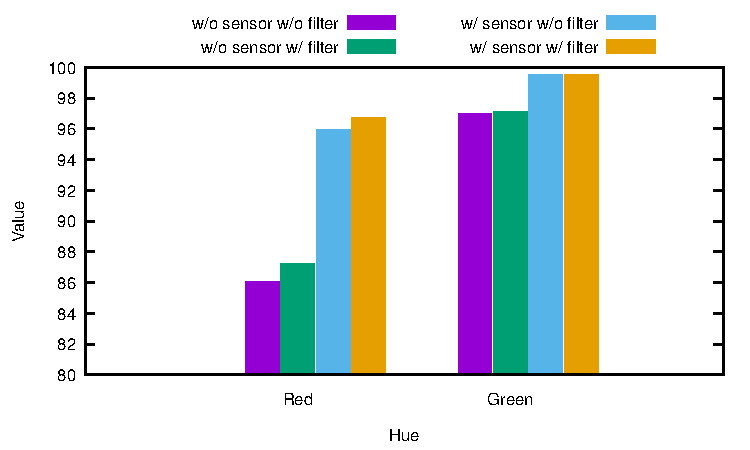
\includegraphics[width=5.2in]{plots/bar_tp.pdf}
\caption{Detection rate for static movement dataset.}
\label{f:tp_stat}
\end{figure}

\ref{f:fp_stat} shows the misdetection rate for the red and green state of traffic lights.
Left one is the false positive detection and the right one is the false negative detection for the traffic light detection.
Here, the false positive count is reduced significantly and false negative is zero.

\begin{figure}[!ht]
\centering
\subfloat[] {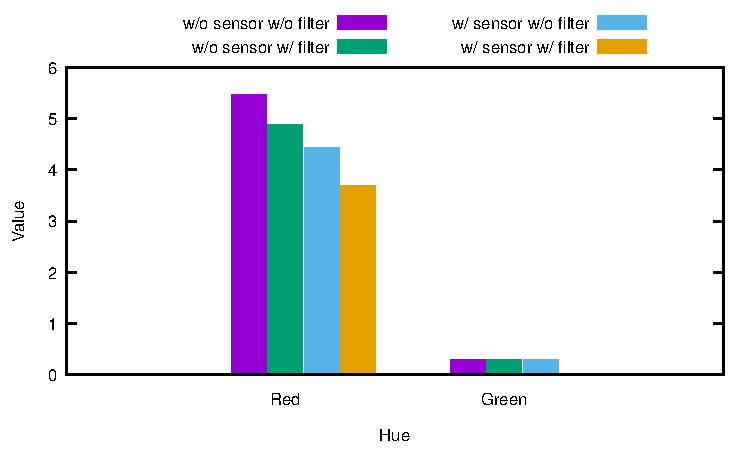
\includegraphics[width=5.2in]{plots/bar_fp.pdf}}

\subfloat[] {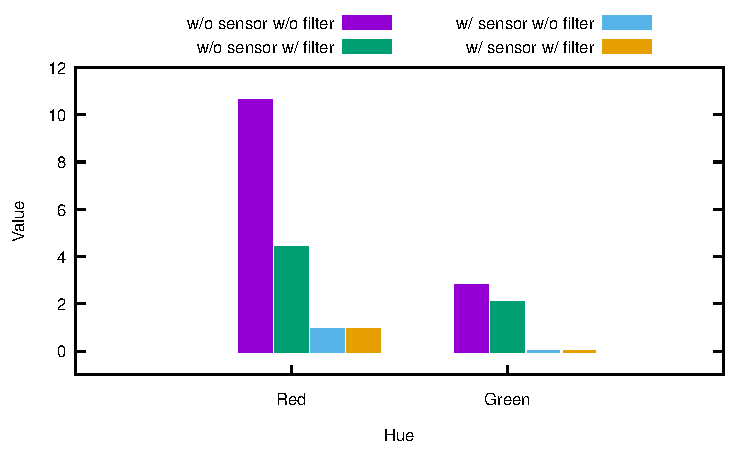
\includegraphics[width=5.2in]{plots/bar_fn.pdf}}
\caption{Misdetection rate for static movement dataset.}
\label{f:fp_stat}
\end{figure}

\ref{t:acc_stat} shows the accuracy rate for our  dataset.
It shows that the average accuracy increases from 91\% to 97\% with sensor hints.

\begin{table}[h!]
  \centering
  \caption{Accuracy for detection in our datasets.}
  \rowcolors{2}{gray!25}{white}
  \label{t:acc_stat}
  \begin{tabular}{  l  r  r r r }
    \rowcolor{gray!50}
    Dataset & w/o sensor & w/o sensor & w/ sensor & w/ sensor \\
    \rowcolor{gray!50}
    name & w/o filter & w/ filter & w/o filter & w/ filter \\
    \hline
    Walking w/sensor (Cloudy day) & 92.21\% & 92.63\% & 95.3229\% & 96.026\% \\
    %Walking w/sensor (Sunny day) & & & \\
    Walking w/sensor (Regular day) & 92.11\% & 92.986\% & 96.16\% & 97.2906\% \\
    Static w/ sensor (Regular day) & 89.7313\% & 90.6142\% & 97.035\% & 98.7908\% \\
    \hline
    Average detection rate & 91.3504\% & 92.0767\% & 97.1726\% & 97.3691\%\\
  \end{tabular}
\end{table}

\section{Evaluation of walk sign detection}
We need the ground truth to classify the walk signs at the video frames.
Accordingly, we annotate the walk sign locations manually at each video frame.
During annotation, we record the position of the walk and stop sign and we label the sign types (walk and stop). 

\begin{table}[ht!]
  \centering
  \caption{Annotated sign in our dataset.}
  \label{t:walk_sign_ann}
  \rowcolors{2}{gray!25}{white}
  \begin{tabular}{  l  c  r r }
    \rowcolor{gray!50}
    Name & Walk sign  & Stop sign \\
    \hline
    Walking w/ sensor (Cloudy day) & 129 & 94 \\ %& 807
    Walking w/ sensor (Regular day) & 68 & 103  \\%& 469
    Total annotated sign & 197 & 197 \\
    \hline
  \end{tabular}
\end{table}

\ref{t:walk_sign_ann} shows the total number of annotated signs in our datasets.
Here, we annotated 394 sign (walk and stop) in total.

We use the multi-layer neural network to classify the signs as we described in \S\ref{s:neural}.
\ref{t:training_neural} shows the length of training and testing dataset for our neural network architecture.
For the training purpose, we use 159 of the walk sign and 151 of the stop sign.
And for testing dataset we use 84 signs in total.

\begin{table}[ht!]
  \centering
  \caption{Training and testing dataset for neural network architecture.}
  \label{t:training_neural}
  \rowcolors{2}{gray!25}{white}
  \begin{tabular}{  l  c  c  r}
    \rowcolor{gray!50}
    Name & Walk sign & Stop sign & Total \\
    \hline
    Training dataset & 159 & 151 & 310\\ %& 807
    Testing dataset & 38 & 46 & 84 \\%& 469
   
    \hline
  \end{tabular}
\end{table}

\subsection{Classifier accuracy for sign detection}

\ref{t:report_walk} shows the final classification results of our neural network classifier.
Here, the average precision for the sign detection is 97.75\% and the average recall we get 97\%.

\begin{table}[h!]
  \centering
  \caption{Classification report for the classifier for sign detection in our dataset.}
  \label{t:report_walk}
  \rowcolors{2}{gray!25}{white}
  \begin{tabular}{  l  c  c  r }
    \rowcolor{gray!50}
     & precision & recall & f1-score \\
    \hline
    Stop sign & 95.5\% & 100\% & 98\% \\
    Walk sign & 100\% & 94\% & 97\% \\
    \hline  
    Average & 97.75\% & 97\% & 97.5\% \\
  \end{tabular}
\end{table}

\ref{t:walk_sign} shows the confusion matrix for the sign detection in our dataset.

\begin{table}[h!]
  \centering
  \caption{Confusion Matrix for sign detection in our dataset.}
  \label{t:walk_sign}
  \rowcolors{2}{gray!25}{white}  
  \begin{tabular}{  l  c  c  r }
    \rowcolor{gray!50}
     & Detected stop sign & Detected walk sign &  \\
    \hline
    Actual stop sign & 46 & 0 & 100\% \\
    Actual walk sign & 2 & 36 & 94.737\% \\
    \hline
    & 95.83\% & 100\% & 97.619\% \\
    
  \end{tabular}
\end{table}

This result shows that for the walk sign we get 2 false detections, while the accuracy for stop sign detection is 100\%.


\section{Evaluation of a public dataset}

In this section, we evaluate our system with a well studied public dataset, LISA Traffic Light Dataset \cite{lisa}.
The LISA Traffic Light Dataset consists of 13 day training clips and 5 night training clips with 4 testing sequences which are captured in San Diego, California, USA \cite{lisa2}.
This dataset has total 46418 frames with 112,971 annotated lights.

The main approach of our system is to use sensor hints to improve the computational time and the detection accuracy.
However, the LISA dataset has no information of the sensor hints, so we manually take the 1/4 of frames approximately.


\begin{figure}[ht!]
  \centering
  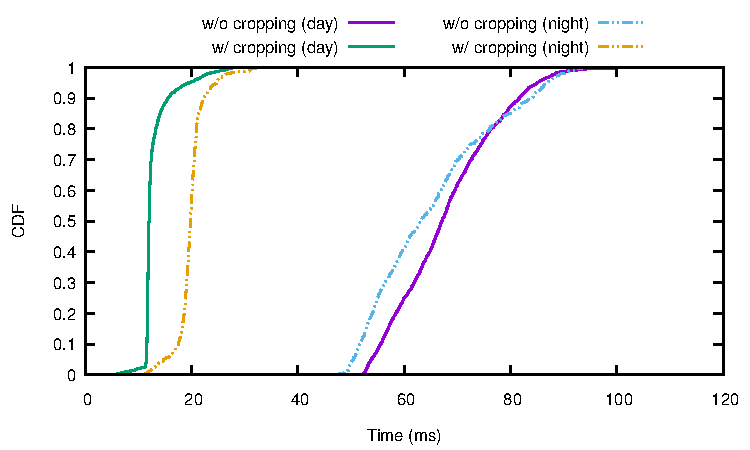
\includegraphics[width=5.2in]{plots/lisacdf.pdf}
  \caption{CDF time of dayClip1 dataset with cropping and without cropping.}
  \label{f:lisa_cdf}
\end{figure}

\ref{f:lisa_cdf} shows the CDF of computation time for dayclip1 dataset with full frames and subframes.
It shows that the median time for full frame is 67.15 ms and for the subframe is 12.03 ms.
We can improve the computation time by 5.58 for this dataset taking the approximate 1/4 of frames.
However, if we have sensor hints we can improve computation time more keeping the subframes area smaller.




\begin{table}[!ht]
  \centering
  \caption{Median computation time (ms) for LISA dataset.}
  \label{t:lisa_time}
  \rowcolors{2}{gray!25}{white}
  \begin{tabular}{  l   r   r  r}
    \rowcolor{gray!50}
    Sequence Nane &  Full frame (ms)  &  Subframe (ms) & Improvement \\
    \hline
    Dayclip-1 & 67.15 & 12.03 & 5.58\% \\
    Dayclip-2 & 53.85 & 10.10 & 5.33\% \\
    Dayclip-3 & 58.63 & 10.81 & 5.42\% \\
    Dayclip-4 & 51.89 & 9.67 & 5.37\% \\
    Dayclip-5 & 68.23 & 13.05 & 5.23\% \\
    Dayclip-6 & 52.24 & 10.01 & 5.22\% \\
    Dayclip-7 & 68.11  & 13.20 & 5.16\% \\
    Dayclip-8 & 52.16  & 9.89  & 5.27\% \\
    Dayclip-9 & 54.22  & 10.40  & 5.21\% \\
    Dayclip-10 & 58.66 & 10.80 & 5.43\% \\
    Dayclip-11 & 53.95 & 10.40 & 5.19\% \\
    Dayclip-12 & 62.50  & 13.05 & 4.79\% \\
    Dayclip-13 & 54.33 & 10.09 & 5.38\% \\
    Nightclip-1 & 63.19 & 19.10 & 3.31\% \\
    Nightclip-2 & 66.48 & 18.55 & 3.58\% \\
    Nightclip-3 & 62.30 & 16.50 & 3.78\% \\
    Nightclip-4 & 60.43 & 13.45 & 4.49\% \\
    Nightclip-5 & 58.89 & 14.50 & 4.06\% \\
    \hline
    Average computation time (ms) & 59.29 & 12.53 & 4.73\% \\
    
  \end{tabular}
\end{table}

\ref{t:lisa_time} shows the median computation time for full frames and subframes for the other clips of LISA dataset.
The last column of \ref{t:lisa_time} shows the improvement of computation time for each dataset.
It shows that the average median computation time for full frame is 59.29 ms and for subframe is 12.53 ms.
Additionally, the average computation time improvement is 4.73\%.


\begin{table}[h!]
  \centering
  \caption{Confusion Matrix without cropping for LISA dataset.}
  \label{t:lisa_con_nocrp}
  \rowcolors{2}{gray!25}{white}
  \begin{tabular}{  l  c  c  r }
    \rowcolor{gray!50}   
     & Detected Red & Detected Green &  \\
    \hline
    Actual Red & 5479 & 2346 & 70.019\% \\
    Actual Green & 1369 & 3682 & 72.896\% \\
    \hline
    & 80.009\% & 61.0816\% & 71.1478\% \\
    
  \end{tabular}
\end{table}

\ref{t:lisa_con_nocrp} shows the confusion matrix for the traffic light decision when we process the full frame for LISA dataset.
\ref{t:lisa_con_crp} shows the confusion matrix cropping approximately the 1/4 of the frame .

\begin{table}[h!]
  \centering
  \caption{Confusion Matrix with cropping for LISA dataset.}
  \label{t:lisa_con_crp}
  \rowcolors{2}{gray!25}{white}
  \begin{tabular}{  l  c  c  r }
    \rowcolor{gray!50}   
     & Detected Red & Detected Green &  \\
    \hline
    Actual Red & 13508 & 2870 & 76\% \\
    Actual Green & 570 & 10588 & 93.3874\% \\
    \hline
    & 94.6824\% & 71.5239\% & 82.8208\% \\
    
  \end{tabular}
\end{table}

This result shows that the red and green traffic light detection is increasing while considering the part of the frames.

\begin{table}[h!]
  \centering
  \caption{Accuracy for detection in LISA datasets.}
  \rowcolors{2}{gray!25}{white}
  \label{t:lisa_acc_stat}
  \begin{tabular}{  l  r  r }
    \rowcolor{gray!50}
    Dataset & Full frame & Sub frame \\
    \hline
    Dayclip-1 & 65.162\% & 77.7014\% \\
    Dayclip-2 & 67.4\% & 76.3948\% \\
    Dayclip-3 & 83.1542\% & 88.7225\% \\
    Dayclip-4 & 77.8626\% & 96.224\% \\
    Dayclip-5 & 84.0831\% & 90.0261\% \\
    Dayclip-6 & 73.1403\% & 83.664\% \\
    Dayclip-10 & 88.6792\% & 97.1698\% \\
    Dayclip-11 & 69.746\% & 79.9209\% \\
    Dayclip-12 & 78.3333\% & 96.6667\% \\
    Dayclip-13 & 68.6257\% & 83.6199\%\\
    \hline
    Average detection rate & 74.1092\% & 87.01574\% \\
  \end{tabular}
\end{table}

\ref{t:lisa_acc_stat} shows the accuracy of traffic light detection for LISA datasets.
Average detection rate is increasing to 87\% from 74\% considering the sub frame.




